\section{Aircraft Configurations}

The methodologies presented in this thesis were developed and demonstrated using two aircraft configurations: the NASA Common Research Model (CRM), and the Generic T-tail Transport (GTT). 

\subsection{NASA Common Research Model}
The NASA CRM is a well-investigated full-configuration aircraft \cite{rivers_further_2012,rivers_experimental_2010} that was developed with the goal of creating a baseline geometry upon which numerous experimental and computational studies could be performed and compared.
It was originally created for the 4th Drag Prediction Workshop \cite{morrison20094th} and was used for the subsequent 5th and 6th editions of the workshop as well \cite{levy2013summary,morrison20166th,roy2017summary,tinoco2017summary}.
The wealth of experimental and computational data lends itself well for the purpose of showcasing the performance of the uncertainty quantification and multi-fidelity data fusion techniques developed in this thesis.

The model was designed by The Boeing Company and is based on the Boeing 777 aircraft with a modified wing. 
It is a conventional tube-wing configuration designed for a cruise Mach number of 0.85.
The NASA CRM was built to be modular such that additional components could be attached to the baseline geometry. 
Consequently, different configurations of the aircraft were tested in the wind tunnel:
\begin{enumerate}
    \item Baseline wing + fuselage model,
    \item Wing + fuselage + pylon and nacelle,
    \item Wing + fuselage + horizontal tail mounted at either $-2^\circ, 0^\circ,$ or $+2^\circ$.
\end{enumerate}
Figure \ref{subfig:nasa_crm_wt_img} shows one such configuration in a wind tunnel. 
For the purpose of this work, the configuration with the wing + fuselage + horizontal tail mounted at $-2^\circ$ is used. 

% \begin{figure}
% \centering
% 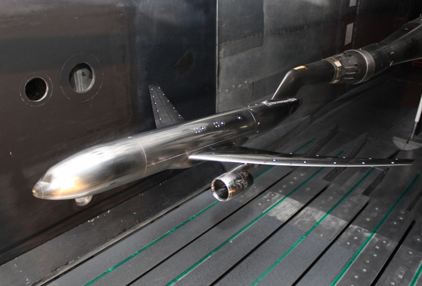
\includegraphics[width=0.75\textwidth]{suthesis/images/nasa_crm_wt.png}
% \caption{NASA CRM wind tunnel model in a wind tunnel. \label{fig:nasa_crm_wt}}
% \end{figure}


\begin{figure}
\center
\subfigure[\label{subfig:nasa_crm_wt_img} NASA Common Research Model]
  {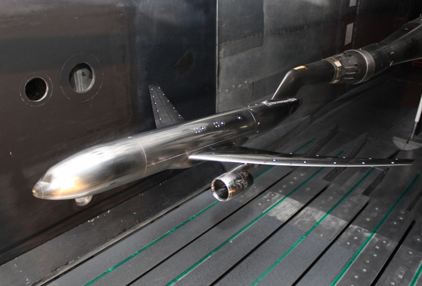
\includegraphics[width=0.48\textwidth]{suthesis/images/nasa_crm_wt.png}}
\subfigure[\label{subfig:gtt_wt_img} Generic T-tail Transport]
  {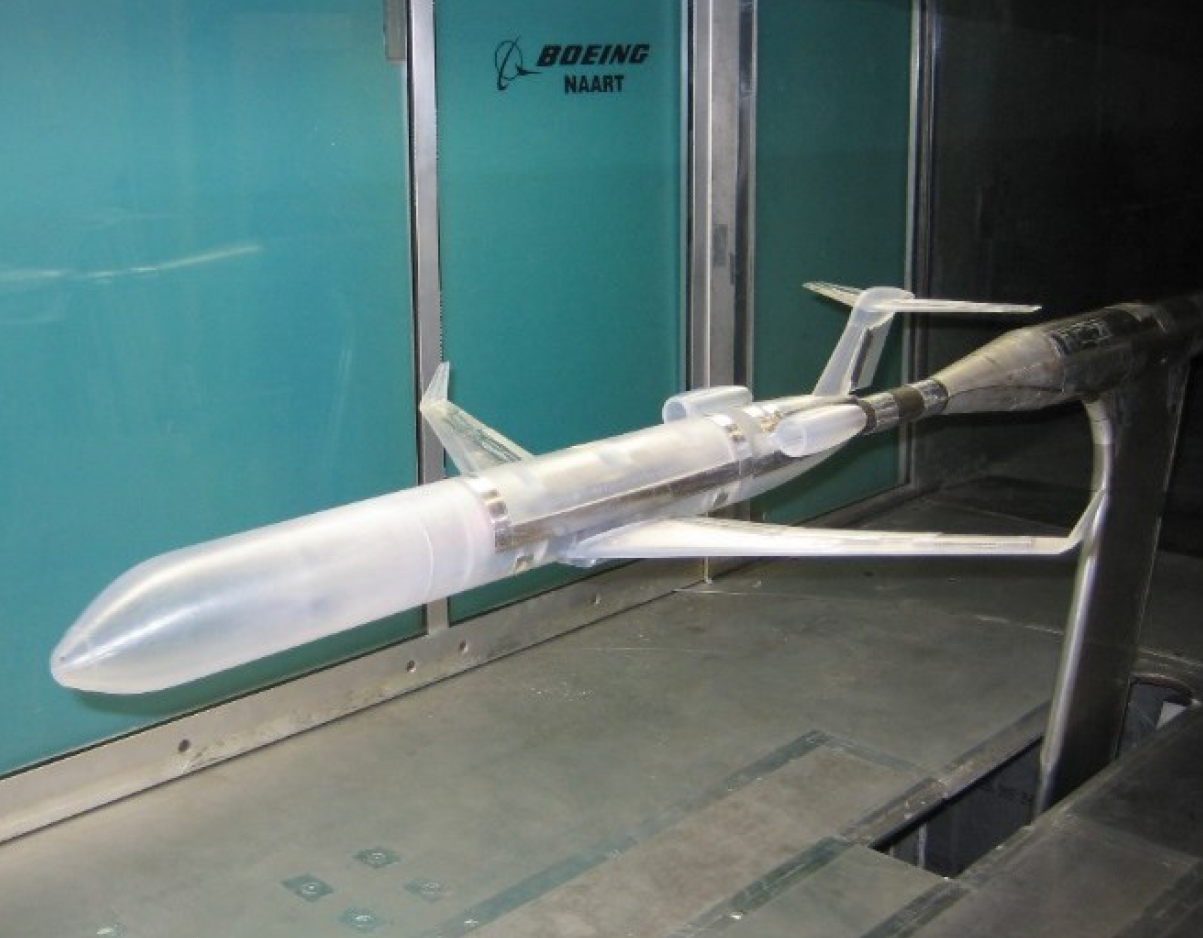
\includegraphics[width=0.48\textwidth, trim=0 92 0 0, clip]{suthesis/images/gtt_naart.png}}
\caption{Wind tunnel models for the two aircraft configurations that are investigated in this work.}\label{fig:aircraft_images}
\end{figure}

\subsection{Generic T-tail Transport}

The GTT aircraft was developed in another collaborative effort between NASA and The Boeing Company. 
The aim of this effort was to provide experimental and computational data to inform a flight simulator that would be used to provide stall recovery training to pilots \cite{cunningham_generic_2018}.
The aircraft configuration is derived from a remotely piloted airplane configuration that was designed by NASA and built by Area-I \cite{kuehme_flight_2014}.
It is a $16\%$ scaled version of the Bombardier CRJ700 which is a currently in-service aircraft.
The configuration is meant to resemble a generic short to medium range single-aisle regional jet with a T-tail and twin aft engines.
Tables \ref{tab:gtt_ref_dim} and \ref{tab:gtt_mass_prop} lists the aerodynamic reference dimensions and the mass properties of the GTT aircraft, respectively.

\begin{table}
\parbox{0.5\textwidth}{
\centering
    \renewcommand{\arraystretch}{1.2}
    \captionsetup{justification=centering}
    \begin{tabular}{|c|c|}
        \hline
        Mean Aerodynamic Chord & $3.374~\mathrm{m}$ \\ \hline
        Wing Span & $23.159~\mathrm{m}$ \\ \hline
        Wing Area & $70.079~\mathrm{m^2}$ \\ \hline
    \end{tabular}
    \caption{Aerodynamic reference dimensions for the GTT aircraft.} 
    \label{tab:gtt_ref_dim}
}
\parbox{0.5\textwidth}{
\centering
    \renewcommand{\arraystretch}{1.2}
    \captionsetup{justification=centering}
    \begin{tabular}{|c|c|}
        \hline
        Weight & $25,332~\mathrm{kg}$ \\ \hline
        $I_{xx}$ & $238,419~\mathrm{kg~m^2}$ \\ \hline
        $I_{yy}$ & $1,510,624~\mathrm{kg~m^2}$ \\ \hline
        $I_{zz}$ & $1,717,539~\mathrm{kg~m^2}$ \\ \hline
    \end{tabular}
    \caption{Mass properties of the GTT aircraft.}
    \label{tab:gtt_mass_prop}
}
\end{table}

The main motivation for using the GTT configuration for this work is the wealth of experimental wind tunnel data that is available \cite{cunningham_preliminary_2018}. 
Three experimental campaigns explored different aspects of the aircraft performance characteristics and were performed in the following facilities:
\begin{enumerate}
    \item NASA Langley Research Center 12-Foot Low-Speed Tunnel (12-Foot LST): Focus on stability derivatives and $\alpha$ sweeps,
    \item Boeing North American Aviation Research Tunnel (NAART): Focus on control derivatives and $\alpha$ and $\beta$ sweeps,
    \item Boeing Flow Visualization Water Tunnel (FVWT): Focus on stability derivatives at various values of $\alpha$.
\end{enumerate}
Figure \ref{subfig:gtt_wt_img} shows the GTT model mounted in the NAART facility.
Only data from the NAART and the FVWT experimental campaigns are used in this work as the data from the 12-Foot LST is a subset of the data from the other two sources. 
Table \ref{tab:gtt_scale_factors} lists the scales of the models used for the various wind tunnel campaigns and for the CFD campaign performed using SU2 for this work. 

\begin{table}
\centering
    \renewcommand{\arraystretch}{1.2}
    \captionsetup{justification=centering}
    \begin{tabular}{|c|c|}
        \hline
        Data Source & Scaling factor \\ \hline
        NASA 12-Foot LST & $0.057$ \\ \hline
        Boeing NAART & $0.020$ \\ \hline
        Boeing FVWT & $0.019$ \\ \hline
        SU2 & $0.158$\\ \hline
    \end{tabular}
    \caption{Scale factors for the different sources of data.}
    \label{tab:gtt_scale_factors}
\end{table}

The NAART and 12-Foot LST models included control surface parts that were individually tested to define the control characteristics of the aircraft. 
The list of control surfaces and their associated deflection ranges is included in Table \ref{tab:gtt_cs_range}.
In addition to these, the entire horizontal stabilizer could be rotated to change the its incidence angle. 
However, since a majority of the wind tunnel tests were performed with the stabilizer mounted at an angle of $-6^\circ$, only that particular incidence angle is used.

\begin{table}
    \renewcommand{\arraystretch}{1.2}
    \centering
    \begin{tabular}{ |c|c| } 
        \hline
        Control Surface & Deflection Range \\ \hline
         Ailerons &  $-25^\circ \leq \delta_a \leq 25^\circ$ \\ \hline
         Elevator &  $-30^\circ \leq \delta_e \leq 30^\circ$ \\ \hline
         Rudder & $0^\circ \leq \delta_r \leq 35^\circ$ \\ \hline
         Flaps & $0^\circ \leq \delta_f \leq 60^\circ$ \\ \hline
         Spoilers & $0^\circ \leq \delta_s \leq 60^\circ$ \\ \hline
    \end{tabular}
    \caption{Control surface deflection ranges for the GTT aircraft.}
    \label{tab:gtt_cs_range}
\end{table}

